\documentclass[crop=false]{standalone}
%\documentclass{standalone}
\usepackage{tikz} % To generate the plot from csv
\usepackage{pgfplots}
\usepackage{graphicx}
\usepackage{booktabs}
\usepackage{subfig}
\usepackage{float}
\usepackage[section]{placeins} % getting figures below sections
\usepackage{blindtext}
\usepackage{siunitx}
\usepgfplotslibrary{units} % Allows to enter the units nicely
\usetikzlibrary{external} %https://tex.stackexchange.com/questions/1460/script-to-automate-externalizing-tikz-graphics
\tikzexternalize[prefix=savedfigures/]

\pgfplotsset{compat=newest} % Allows to place the legend below plot
\usepackage{pgfplotstable}
\usepgfplotslibrary{statistics}

% #################### Function definition for box plots read table ##################\
\makeatletter
\pgfplotsset{
	boxplot prepared from table/.code={
		\def\tikz@plot@handler{\pgfplotsplothandlerboxplotprepared}%
		\pgfplotsset{
			/pgfplots/boxplot prepared from table/.cd,
			#1,
		}
	},
	/pgfplots/boxplot prepared from table/.cd,
	table/.code={\pgfplotstablecopy{#1}\to\boxplot@datatable},
	row/.initial=0,
	make style readable from table/.style={
		#1/.code={
			\pgfplotstablegetelem{\pgfkeysvalueof{/pgfplots/boxplot prepared from table/row}}{##1}\of\boxplot@datatable
			\pgfplotsset{boxplot/#1/.expand once={\pgfplotsretval}}
		}
	},
	make style readable from table=lower whisker,
	make style readable from table=upper whisker,
	make style readable from table=lower quartile,
	make style readable from table=upper quartile,
	make style readable from table=median,
	make style readable from table=average,
	make style readable from table=lower notch,
	make style readable from table=upper notch
}
\makeatother
\begin{document}
\pgfkeys{/pgf/number format/.cd,1000 sep={\,}}

\section{33 3 Mumford1 SA ALL param 20210818 115649}

% ######################## UTRP SA Cooling rate ######################## 
\begin{figure} 
\centering 
\tikzsetnextfilename{UTRP_DBMOSA_BP_cooling_rate} 
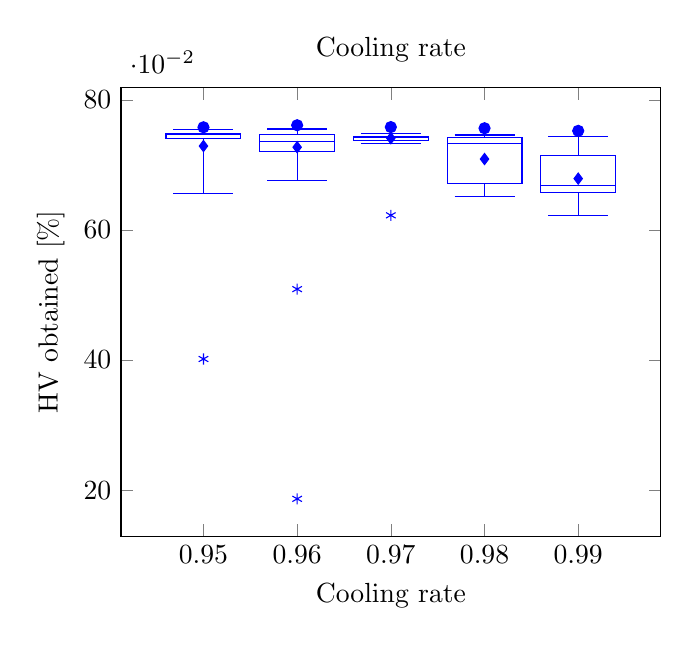
\begin{tikzpicture} 
\begin{axis}[ 
title={Cooling rate}, 
boxplot/draw direction=y, 
xtick={1,2,3,4,5}, 
xticklabels={0.95,0.96,0.97,0.98,0.99}, 
x tick label style={rotate=0, align=center}, 
xlabel={Cooling rate}, 
% y tick label style={/pgf/number format/.cd,fixed,precision=3, zerofill}, 
scaled y ticks={base 10:2}, 
ylabel={HV obtained [\%]}, 
] 

% ############## Cooling_rate=0.95 ################## 
\addplot[boxplot, mark=asterisk, 
boxplot prepared={ 
lower whisker=0.65617, 
upper whisker=0.75393, 
lower quartile=0.74027, 
upper quartile=0.74752, 
median=0.74641, 
average=0.72903}, 
color = blue, solid, area legend] 
coordinates {
(1,0.40161)}; 
\addplot[only marks,mark=*,color = blue]coordinates{(1,0.7579)}; 

% ############## Cooling_rate=0.96 ################## 
\addplot[boxplot, mark=asterisk, 
boxplot prepared={ 
lower whisker=0.6765, 
upper whisker=0.75523, 
lower quartile=0.72044, 
upper quartile=0.74623, 
median=0.73548, 
average=0.72726}, 
color = blue, solid, area legend] 
coordinates {
(2,0.18656)
(2,0.50904)}; 
\addplot[only marks,mark=*,color = blue]coordinates{(2,0.76103)}; 

% ############## Cooling_rate=0.97 ################## 
\addplot[boxplot, mark=asterisk, 
boxplot prepared={ 
lower whisker=0.73348, 
upper whisker=0.74777, 
lower quartile=0.73767, 
upper quartile=0.74349, 
median=0.74247, 
average=0.74108}, 
color = blue, solid, area legend] 
coordinates {
(3,0.6225)}; 
\addplot[only marks,mark=*,color = blue]coordinates{(3,0.7582)}; 

% ############## Cooling_rate=0.98 ################## 
\addplot[boxplot, mark=asterisk, 
boxplot prepared={ 
lower whisker=0.65153, 
upper whisker=0.74601, 
lower quartile=0.67091, 
upper quartile=0.74175, 
median=0.73324, 
average=0.70909}, 
color = blue, solid, area legend] 
coordinates {}; 
\addplot[only marks,mark=*,color = blue]coordinates{(4,0.75643)}; 

% ############## Cooling_rate=0.99 ################## 
\addplot[boxplot, mark=asterisk, 
boxplot prepared={ 
lower whisker=0.62204, 
upper whisker=0.74408, 
lower quartile=0.65744, 
upper quartile=0.71417, 
median=0.66856, 
average=0.67891}, 
color = blue, solid, area legend] 
coordinates {}; 
\addplot[only marks,mark=*,color = blue]coordinates{(5,0.75241)}; 

\end{axis}
\end{tikzpicture}
\end{figure} 

% ######################## UTRP SA Maximum attempts ######################## 
\begin{figure} 
\centering 
\tikzsetnextfilename{UTRP_DBMOSA_BP_max_attempts} 
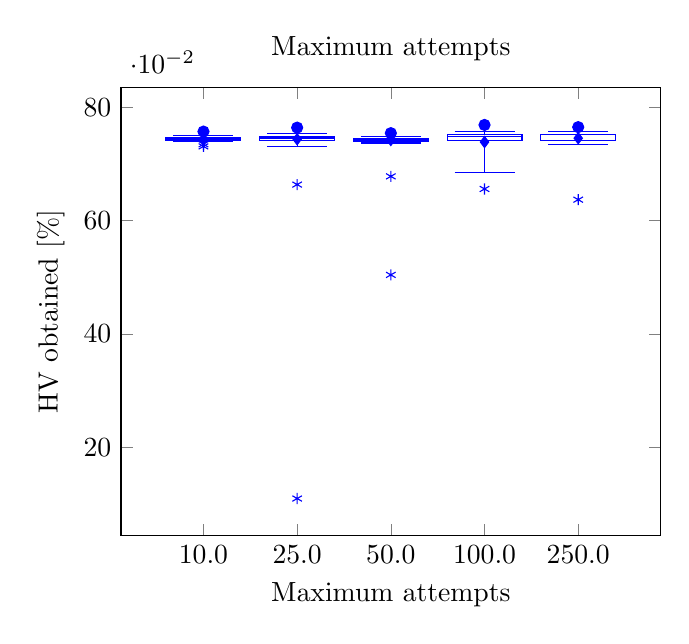
\begin{tikzpicture} 
\begin{axis}[ 
title={Maximum attempts}, 
boxplot/draw direction=y, 
xtick={1,2,3,4,5}, 
xticklabels={10.0,25.0,50.0,100.0,250.0}, 
x tick label style={rotate=0, align=center}, 
xlabel={Maximum attempts}, 
% y tick label style={/pgf/number format/.cd,fixed,precision=3, zerofill}, 
scaled y ticks={base 10:2}, 
ylabel={HV obtained [\%]}, 
] 

% ############## max_attempts=10.0 ################## 
\addplot[boxplot, mark=asterisk, 
boxplot prepared={ 
lower whisker=0.7405, 
upper whisker=0.74974, 
lower quartile=0.74144, 
upper quartile=0.74588, 
median=0.74254, 
average=0.74399}, 
color = blue, solid, area legend] 
coordinates {
(1,0.7349)
(1,0.73115)}; 
\addplot[only marks,mark=*,color = blue]coordinates{(1,0.75732)}; 

% ############## max_attempts=25.0 ################## 
\addplot[boxplot, mark=asterisk, 
boxplot prepared={ 
lower whisker=0.73032, 
upper whisker=0.75462, 
lower quartile=0.74098, 
upper quartile=0.74837, 
median=0.74598, 
average=0.74378}, 
color = blue, solid, area legend] 
coordinates {
(2,0.66372)
(2,0.10931)}; 
\addplot[only marks,mark=*,color = blue]coordinates{(2,0.7643)}; 

% ############## max_attempts=50.0 ################## 
\addplot[boxplot, mark=asterisk, 
boxplot prepared={ 
lower whisker=0.73714, 
upper whisker=0.74885, 
lower quartile=0.73909, 
upper quartile=0.74462, 
median=0.74244, 
average=0.74244}, 
color = blue, solid, area legend] 
coordinates {
(3,0.50423)
(3,0.67822)}; 
\addplot[only marks,mark=*,color = blue]coordinates{(3,0.75454)}; 

% ############## max_attempts=100.0 ################## 
\addplot[boxplot, mark=asterisk, 
boxplot prepared={ 
lower whisker=0.68498, 
upper whisker=0.75675, 
lower quartile=0.74092, 
upper quartile=0.75249, 
median=0.74819, 
average=0.73884}, 
color = blue, solid, area legend] 
coordinates {
(4,0.65597)}; 
\addplot[only marks,mark=*,color = blue]coordinates{(4,0.76906)}; 

% ############## max_attempts=250.0 ################## 
\addplot[boxplot, mark=asterisk, 
boxplot prepared={ 
lower whisker=0.73417, 
upper whisker=0.75711, 
lower quartile=0.741, 
upper quartile=0.75222, 
median=0.74232, 
average=0.74563}, 
color = blue, solid, area legend] 
coordinates {
(5,0.63706)}; 
\addplot[only marks,mark=*,color = blue]coordinates{(5,0.76517)}; 

\end{axis}
\end{tikzpicture}
\end{figure} 

% ######################## UTRP SA Max iterations per epoch ######################## 
\begin{figure} 
\centering 
\tikzsetnextfilename{UTRP_DBMOSA_BP_max_iterations_per_epoch} 
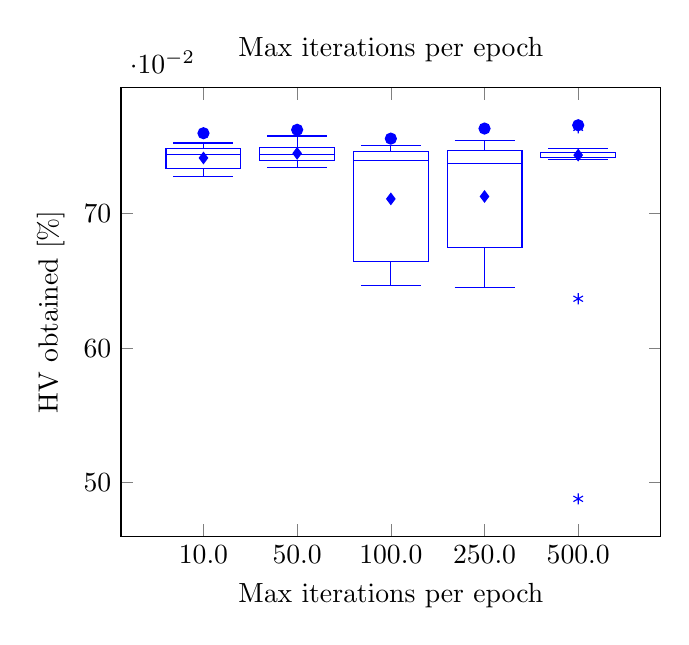
\begin{tikzpicture} 
\begin{axis}[ 
title={Max iterations per epoch}, 
boxplot/draw direction=y, 
xtick={1,2,3,4,5}, 
xticklabels={10.0,50.0,100.0,250.0,500.0}, 
x tick label style={rotate=0, align=center}, 
xlabel={Max iterations per epoch}, 
% y tick label style={/pgf/number format/.cd,fixed,precision=3, zerofill}, 
scaled y ticks={base 10:2}, 
ylabel={HV obtained [\%]}, 
] 

% ############## max_iterations_t=10.0 ################## 
\addplot[boxplot, mark=asterisk, 
boxplot prepared={ 
lower whisker=0.72727, 
upper whisker=0.75242, 
lower quartile=0.7334, 
upper quartile=0.74807, 
median=0.74409, 
average=0.74128}, 
color = blue, solid, area legend] 
coordinates {}; 
\addplot[only marks,mark=*,color = blue]coordinates{(1,0.75968)}; 

% ############## max_iterations_t=50.0 ################## 
\addplot[boxplot, mark=asterisk, 
boxplot prepared={ 
lower whisker=0.73438, 
upper whisker=0.75765, 
lower quartile=0.73925, 
upper quartile=0.74924, 
median=0.74414, 
average=0.74473}, 
color = blue, solid, area legend] 
coordinates {}; 
\addplot[only marks,mark=*,color = blue]coordinates{(2,0.76221)}; 

% ############## max_iterations_t=100.0 ################## 
\addplot[boxplot, mark=asterisk, 
boxplot prepared={ 
lower whisker=0.64672, 
upper whisker=0.75042, 
lower quartile=0.66445, 
upper quartile=0.74588, 
median=0.73934, 
average=0.7109}, 
color = blue, solid, area legend] 
coordinates {}; 
\addplot[only marks,mark=*,color = blue]coordinates{(3,0.75567)}; 

% ############## max_iterations_t=250.0 ################## 
\addplot[boxplot, mark=asterisk, 
boxplot prepared={ 
lower whisker=0.64531, 
upper whisker=0.75398, 
lower quartile=0.67491, 
upper quartile=0.74682, 
median=0.73731, 
average=0.71269}, 
color = blue, solid, area legend] 
coordinates {}; 
\addplot[only marks,mark=*,color = blue]coordinates{(4,0.76315)}; 

% ############## max_iterations_t=500.0 ################## 
\addplot[boxplot, mark=asterisk, 
boxplot prepared={ 
lower whisker=0.73989, 
upper whisker=0.74852, 
lower quartile=0.74149, 
upper quartile=0.74551, 
median=0.74162, 
average=0.74343}, 
color = blue, solid, area legend] 
coordinates {
(5,0.76364)
(5,0.488)
(5,0.63669)}; 
\addplot[only marks,mark=*,color = blue]coordinates{(5,0.76561)}; 

\end{axis}
\end{tikzpicture}
\end{figure} 

% ######################## UTRP SA Maximum poor epochs ######################## 
\begin{figure} 
\centering 
\tikzsetnextfilename{UTRP_DBMOSA_BP_max_poor_epochs} 
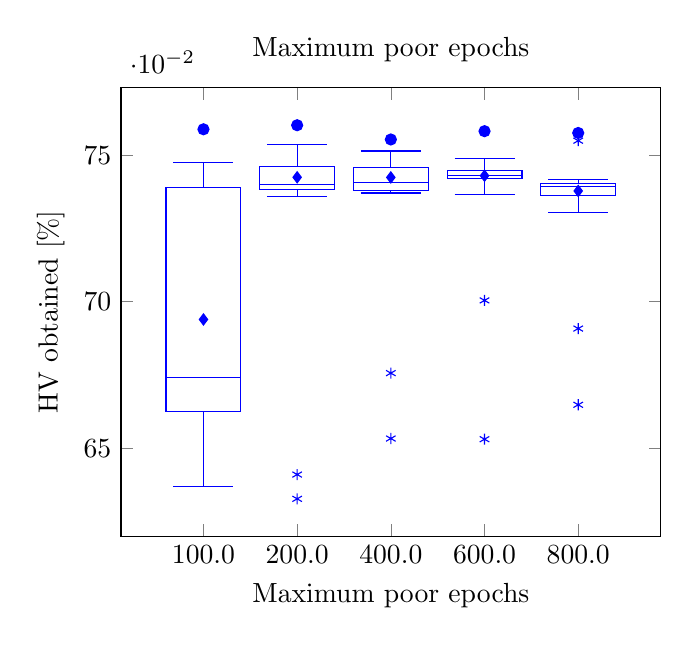
\begin{tikzpicture} 
\begin{axis}[ 
title={Maximum poor epochs}, 
boxplot/draw direction=y, 
xtick={1,2,3,4,5}, 
xticklabels={100.0,200.0,400.0,600.0,800.0}, 
x tick label style={rotate=0, align=center}, 
xlabel={Maximum poor epochs}, 
% y tick label style={/pgf/number format/.cd,fixed,precision=3, zerofill}, 
scaled y ticks={base 10:2}, 
ylabel={HV obtained [\%]}, 
] 

% ############## max_poor_epochs=100.0 ################## 
\addplot[boxplot, mark=asterisk, 
boxplot prepared={ 
lower whisker=0.63684, 
upper whisker=0.7475, 
lower quartile=0.66265, 
upper quartile=0.73912, 
median=0.67418, 
average=0.69394}, 
color = blue, solid, area legend] 
coordinates {}; 
\addplot[only marks,mark=*,color = blue]coordinates{(1,0.75884)}; 

% ############## max_poor_epochs=200.0 ################## 
\addplot[boxplot, mark=asterisk, 
boxplot prepared={ 
lower whisker=0.73576, 
upper whisker=0.75358, 
lower quartile=0.73816, 
upper quartile=0.74607, 
median=0.73986, 
average=0.74244}, 
color = blue, solid, area legend] 
coordinates {
(2,0.641)
(2,0.63271)}; 
\addplot[only marks,mark=*,color = blue]coordinates{(2,0.76022)}; 

% ############## max_poor_epochs=400.0 ################## 
\addplot[boxplot, mark=asterisk, 
boxplot prepared={ 
lower whisker=0.73708, 
upper whisker=0.75142, 
lower quartile=0.73809, 
upper quartile=0.74576, 
median=0.74077, 
average=0.74241}, 
color = blue, solid, area legend] 
coordinates {
(3,0.6533)
(3,0.67562)}; 
\addplot[only marks,mark=*,color = blue]coordinates{(3,0.75536)}; 

% ############## max_poor_epochs=600.0 ################## 
\addplot[boxplot, mark=asterisk, 
boxplot prepared={ 
lower whisker=0.73643, 
upper whisker=0.74877, 
lower quartile=0.74198, 
upper quartile=0.74472, 
median=0.74312, 
average=0.743}, 
color = blue, solid, area legend] 
coordinates {
(4,0.65306)
(4,0.70043)}; 
\addplot[only marks,mark=*,color = blue]coordinates{(4,0.75819)}; 

% ############## max_poor_epochs=800.0 ################## 
\addplot[boxplot, mark=asterisk, 
boxplot prepared={ 
lower whisker=0.73057, 
upper whisker=0.7418, 
lower quartile=0.73625, 
upper quartile=0.74024, 
median=0.73923, 
average=0.73779}, 
color = blue, solid, area legend] 
coordinates {
(5,0.69083)
(5,0.66481)
(5,0.75494)}; 
\addplot[only marks,mark=*,color = blue]coordinates{(5,0.75758)}; 

\end{axis}
\end{tikzpicture}
\end{figure} 

% ######################## UTRP SA Maximum reheating times ######################## 
\begin{figure} 
\centering 
\tikzsetnextfilename{UTRP_DBMOSA_BP_max_reheating_times} 
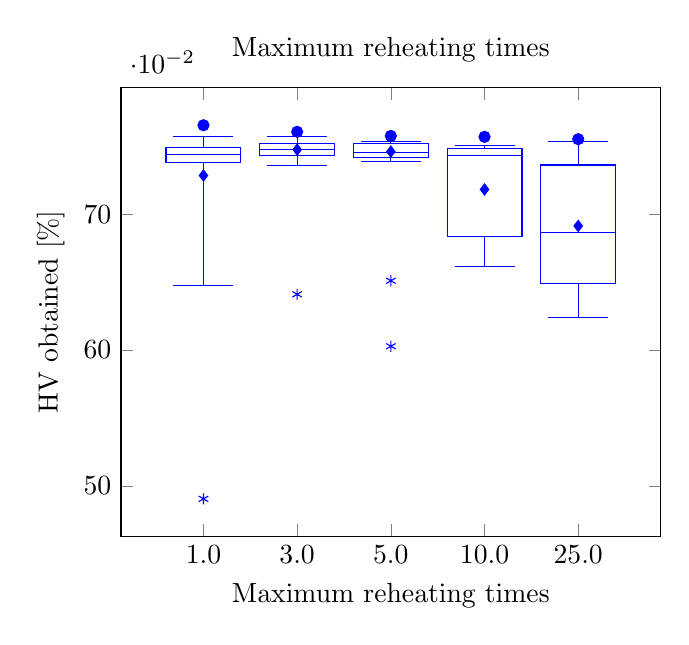
\begin{tikzpicture} 
\begin{axis}[ 
title={Maximum reheating times}, 
boxplot/draw direction=y, 
xtick={1,2,3,4,5}, 
xticklabels={1.0,3.0,5.0,10.0,25.0}, 
x tick label style={rotate=0, align=center}, 
xlabel={Maximum reheating times}, 
% y tick label style={/pgf/number format/.cd,fixed,precision=3, zerofill}, 
scaled y ticks={base 10:2}, 
ylabel={HV obtained [\%]}, 
] 

% ############## max_reheating_times=1.0 ################## 
\addplot[boxplot, mark=asterisk, 
boxplot prepared={ 
lower whisker=0.64781, 
upper whisker=0.75724, 
lower quartile=0.73817, 
upper quartile=0.74926, 
median=0.74369, 
average=0.72848}, 
color = blue, solid, area legend] 
coordinates {
(1,0.49052)}; 
\addplot[only marks,mark=*,color = blue]coordinates{(1,0.76544)}; 

% ############## max_reheating_times=3.0 ################## 
\addplot[boxplot, mark=asterisk, 
boxplot prepared={ 
lower whisker=0.73613, 
upper whisker=0.75692, 
lower quartile=0.74325, 
upper quartile=0.75174, 
median=0.74753, 
average=0.74747}, 
color = blue, solid, area legend] 
coordinates {
(2,0.641)}; 
\addplot[only marks,mark=*,color = blue]coordinates{(2,0.76059)}; 

% ############## max_reheating_times=5.0 ################## 
\addplot[boxplot, mark=asterisk, 
boxplot prepared={ 
lower whisker=0.73864, 
upper whisker=0.75322, 
lower quartile=0.74156, 
upper quartile=0.75208, 
median=0.74519, 
average=0.74605}, 
color = blue, solid, area legend] 
coordinates {
(3,0.6028)
(3,0.65101)}; 
\addplot[only marks,mark=*,color = blue]coordinates{(3,0.75759)}; 

% ############## max_reheating_times=10.0 ################## 
\addplot[boxplot, mark=asterisk, 
boxplot prepared={ 
lower whisker=0.66135, 
upper whisker=0.75058, 
lower quartile=0.68325, 
upper quartile=0.74802, 
median=0.74312, 
average=0.71819}, 
color = blue, solid, area legend] 
coordinates {}; 
\addplot[only marks,mark=*,color = blue]coordinates{(4,0.7569)}; 

% ############## max_reheating_times=25.0 ################## 
\addplot[boxplot, mark=asterisk, 
boxplot prepared={ 
lower whisker=0.62422, 
upper whisker=0.75363, 
lower quartile=0.64881, 
upper quartile=0.73618, 
median=0.6863, 
average=0.69134}, 
color = blue, solid, area legend] 
coordinates {}; 
\addplot[only marks,mark=*,color = blue]coordinates{(5,0.75519)}; 

\end{axis}
\end{tikzpicture}
\end{figure} 

% ######################## UTRP SA Minimum accepts ######################## 
\begin{figure} 
\centering 
\tikzsetnextfilename{UTRP_DBMOSA_BP_min_accepts} 
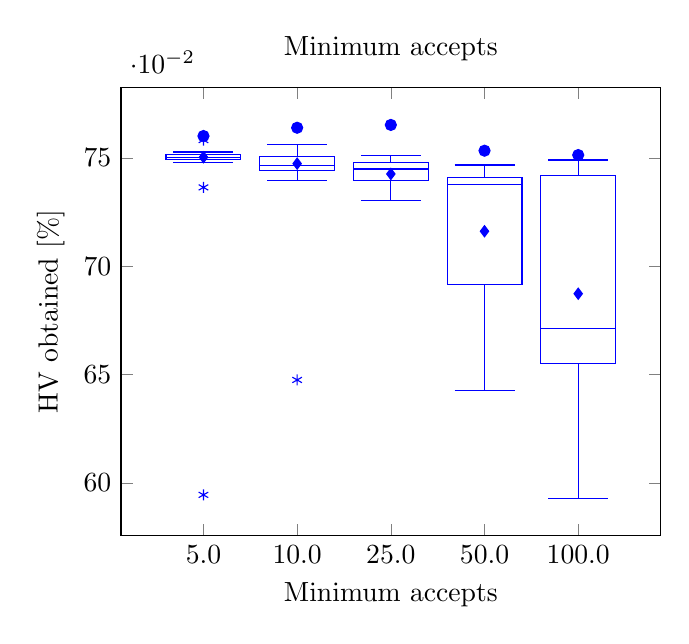
\begin{tikzpicture} 
\begin{axis}[ 
title={Minimum accepts}, 
boxplot/draw direction=y, 
xtick={1,2,3,4,5}, 
xticklabels={5.0,10.0,25.0,50.0,100.0}, 
x tick label style={rotate=0, align=center}, 
xlabel={Minimum accepts}, 
% y tick label style={/pgf/number format/.cd,fixed,precision=3, zerofill}, 
scaled y ticks={base 10:2}, 
ylabel={HV obtained [\%]}, 
] 

% ############## min_accepts=5.0 ################## 
\addplot[boxplot, mark=asterisk, 
boxplot prepared={ 
lower whisker=0.74791, 
upper whisker=0.75276, 
lower quartile=0.74933, 
upper quartile=0.75152, 
median=0.75002, 
average=0.75034}, 
color = blue, solid, area legend] 
coordinates {
(1,0.73641)
(1,0.59442)
(1,0.75827)}; 
\addplot[only marks,mark=*,color = blue]coordinates{(1,0.76014)}; 

% ############## min_accepts=10.0 ################## 
\addplot[boxplot, mark=asterisk, 
boxplot prepared={ 
lower whisker=0.73959, 
upper whisker=0.7561, 
lower quartile=0.74423, 
upper quartile=0.7506, 
median=0.74648, 
average=0.74738}, 
color = blue, solid, area legend] 
coordinates {
(2,0.64749)}; 
\addplot[only marks,mark=*,color = blue]coordinates{(2,0.76396)}; 

% ############## min_accepts=25.0 ################## 
\addplot[boxplot, mark=asterisk, 
boxplot prepared={ 
lower whisker=0.73045, 
upper whisker=0.75097, 
lower quartile=0.73974, 
upper quartile=0.74781, 
median=0.74491, 
average=0.7426}, 
color = blue, solid, area legend] 
coordinates {}; 
\addplot[only marks,mark=*,color = blue]coordinates{(3,0.76526)}; 

% ############## min_accepts=50.0 ################## 
\addplot[boxplot, mark=asterisk, 
boxplot prepared={ 
lower whisker=0.64255, 
upper whisker=0.74676, 
lower quartile=0.69168, 
upper quartile=0.74102, 
median=0.73793, 
average=0.71616}, 
color = blue, solid, area legend] 
coordinates {}; 
\addplot[only marks,mark=*,color = blue]coordinates{(4,0.75336)}; 

% ############## min_accepts=100.0 ################## 
\addplot[boxplot, mark=asterisk, 
boxplot prepared={ 
lower whisker=0.59273, 
upper whisker=0.74908, 
lower quartile=0.65521, 
upper quartile=0.74209, 
median=0.67106, 
average=0.68731}, 
color = blue, solid, area legend] 
coordinates {}; 
\addplot[only marks,mark=*,color = blue]coordinates{(5,0.75135)}; 

\end{axis}
\end{tikzpicture}
\end{figure} 

% ######################## UTRP SA Reheating rate ######################## 
\begin{figure} 
\centering 
\tikzsetnextfilename{UTRP_DBMOSA_BP_reheating_rate} 
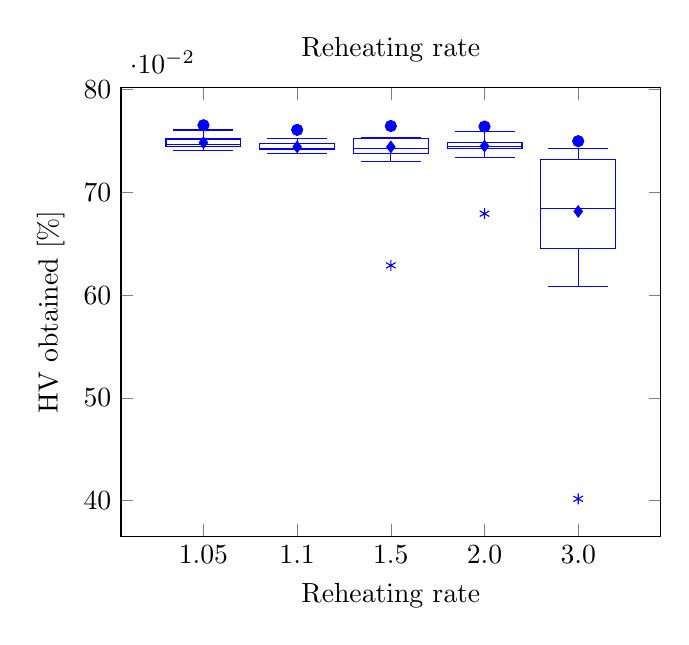
\begin{tikzpicture} 
\begin{axis}[ 
title={Reheating rate}, 
boxplot/draw direction=y, 
xtick={1,2,3,4,5}, 
xticklabels={1.05,1.1,1.5,2.0,3.0}, 
x tick label style={rotate=0, align=center}, 
xlabel={Reheating rate}, 
% y tick label style={/pgf/number format/.cd,fixed,precision=3, zerofill}, 
scaled y ticks={base 10:2}, 
ylabel={HV obtained [\%]}, 
] 

% ############## Reheating_rate=1.05 ################## 
\addplot[boxplot, mark=asterisk, 
boxplot prepared={ 
lower whisker=0.74065, 
upper whisker=0.76072, 
lower quartile=0.74443, 
upper quartile=0.75196, 
median=0.7466, 
average=0.74847}, 
color = blue, solid, area legend] 
coordinates {}; 
\addplot[only marks,mark=*,color = blue]coordinates{(1,0.76538)}; 

% ############## Reheating_rate=1.1 ################## 
\addplot[boxplot, mark=asterisk, 
boxplot prepared={ 
lower whisker=0.73822, 
upper whisker=0.75272, 
lower quartile=0.74191, 
upper quartile=0.74733, 
median=0.74289, 
average=0.74434}, 
color = blue, solid, area legend] 
coordinates {}; 
\addplot[only marks,mark=*,color = blue]coordinates{(2,0.76085)}; 

% ############## Reheating_rate=1.5 ################## 
\addplot[boxplot, mark=asterisk, 
boxplot prepared={ 
lower whisker=0.72969, 
upper whisker=0.75384, 
lower quartile=0.73806, 
upper quartile=0.75242, 
median=0.74293, 
average=0.7443}, 
color = blue, solid, area legend] 
coordinates {
(3,0.62894)}; 
\addplot[only marks,mark=*,color = blue]coordinates{(3,0.76462)}; 

% ############## Reheating_rate=2.0 ################## 
\addplot[boxplot, mark=asterisk, 
boxplot prepared={ 
lower whisker=0.73373, 
upper whisker=0.75968, 
lower quartile=0.74297, 
upper quartile=0.74814, 
median=0.74479, 
average=0.74511}, 
color = blue, solid, area legend] 
coordinates {
(4,0.67926)}; 
\addplot[only marks,mark=*,color = blue]coordinates{(4,0.7641)}; 

% ############## Reheating_rate=3.0 ################## 
\addplot[boxplot, mark=asterisk, 
boxplot prepared={ 
lower whisker=0.608, 
upper whisker=0.74304, 
lower quartile=0.64497, 
upper quartile=0.73231, 
median=0.6839, 
average=0.68141}, 
color = blue, solid, area legend] 
coordinates {
(5,0.40168)}; 
\addplot[only marks,mark=*,color = blue]coordinates{(5,0.7499)}; 

\end{axis}
\end{tikzpicture}
\end{figure} 

% ######################## UTRP SA Starting temperature ######################## 
\begin{figure} 
\centering 
\tikzsetnextfilename{UTRP_DBMOSA_BP_initial_temp} 
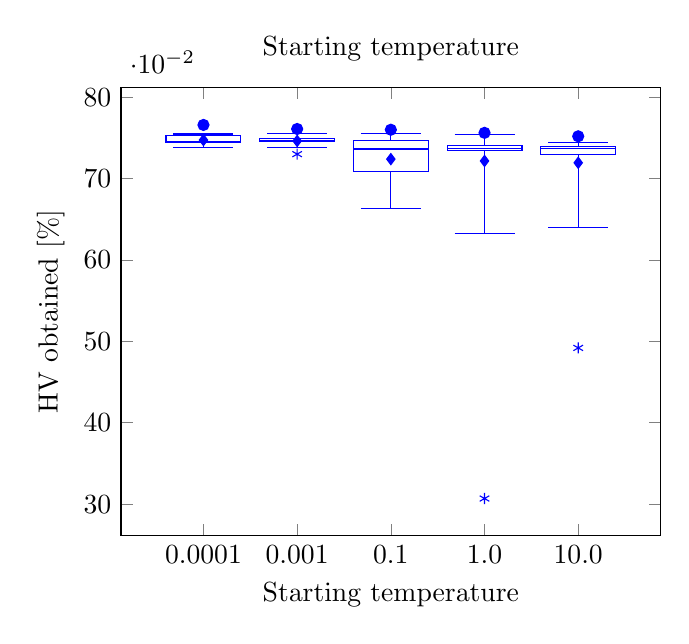
\begin{tikzpicture} 
\begin{axis}[ 
title={Starting temperature}, 
boxplot/draw direction=y, 
xtick={1,2,3,4,5}, 
xticklabels={0.0001,0.001,0.1,1.0,10.0}, 
x tick label style={rotate=0, align=center}, 
xlabel={Starting temperature}, 
% y tick label style={/pgf/number format/.cd,fixed,precision=3, zerofill}, 
scaled y ticks={base 10:2}, 
ylabel={HV obtained [\%]}, 
] 

% ############## Temp=0.0001 ################## 
\addplot[boxplot, mark=asterisk, 
boxplot prepared={ 
lower whisker=0.73762, 
upper whisker=0.7547, 
lower quartile=0.74377, 
upper quartile=0.75266, 
median=0.74598, 
average=0.74728}, 
color = blue, solid, area legend] 
coordinates {}; 
\addplot[only marks,mark=*,color = blue]coordinates{(1,0.76585)}; 

% ############## Temp=0.001 ################## 
\addplot[boxplot, mark=asterisk, 
boxplot prepared={ 
lower whisker=0.73819, 
upper whisker=0.75498, 
lower quartile=0.74533, 
upper quartile=0.74878, 
median=0.74655, 
average=0.74618}, 
color = blue, solid, area legend] 
coordinates {
(2,0.72997)}; 
\addplot[only marks,mark=*,color = blue]coordinates{(2,0.76087)}; 

% ############## Temp=0.1 ################## 
\addplot[boxplot, mark=asterisk, 
boxplot prepared={ 
lower whisker=0.6631, 
upper whisker=0.75485, 
lower quartile=0.70887, 
upper quartile=0.74711, 
median=0.73625, 
average=0.72382}, 
color = blue, solid, area legend] 
coordinates {}; 
\addplot[only marks,mark=*,color = blue]coordinates{(3,0.75995)}; 

% ############## Temp=1.0 ################## 
\addplot[boxplot, mark=asterisk, 
boxplot prepared={ 
lower whisker=0.6326, 
upper whisker=0.75422, 
lower quartile=0.73479, 
upper quartile=0.74046, 
median=0.73734, 
average=0.72156}, 
color = blue, solid, area legend] 
coordinates {
(4,0.30684)}; 
\addplot[only marks,mark=*,color = blue]coordinates{(4,0.75614)}; 

% ############## Temp=10.0 ################## 
\addplot[boxplot, mark=asterisk, 
boxplot prepared={ 
lower whisker=0.64015, 
upper whisker=0.7444, 
lower quartile=0.72899, 
upper quartile=0.73901, 
median=0.73646, 
average=0.71932}, 
color = blue, solid, area legend] 
coordinates {
(5,0.4919)}; 
\addplot[only marks,mark=*,color = blue]coordinates{(5,0.75189)}; 

\end{axis}
\end{tikzpicture}
\end{figure} 
\begin{table}
\centering
\caption{Legend for the boxplot.}
\begin{tabular}{ll}
\toprule
 Index &  Name \\
\midrule
     0 &    10 \\
     1 &    50 \\
     2 &   100 \\
     3 &   250 \\
     4 &   500 \\
\bottomrule
\end{tabular}
\end{table}

\end{document}
